\subsubsection{Attention and transformers}
\label{sub:attention_and_transformers}

In their paper `Attention is all you need'~\footcite{DBLP:journals/corr/VaswaniSPUJGKP17} Google researchers around Ashish Vaswani introduced a new architecture reliant solely on attention mechanisms, i.e. without any recurrence or convolution. Nonetheless, this `transformer' based architecture is superior in both quality and speed. Its structure allows for strong parallelization and thus requires significantly less time to train. Furthermore, transformers generalize well to other tasks, so that the same model can be utilized for multiple \gls{nlp} tasks.
In the following self-attention and other shit will be presented which are important for the transformer architecture.

\paragraph{Self-attention}
Given are a sequence of input vectors $ \boldsymbol{x_1}, \boldsymbol{x_2}, \dots, \boldsymbol{x_t} $ and corresponding output vectors $ \boldsymbol{y_1}, \boldsymbol{y_2}, \dots, \boldsymbol{y_t} $, all of which have dimension $ k $. For the calculation of the output vector $ \boldsymbol{y_i} $, the self-attention mechanism takes a weighted average over all the input vectors
\begin{equation}
	\boldsymbol{y_i} = \sum_j w_{ij} \boldsymbol{x}_j
\end{equation}
where $ j $ indexes over the input sequence the sum of all weights is equal to $ 1 $. Unlike in other architectures, $ w_{ij} $ is not a parameter, but it is the result of a function over $ \boldsymbol{x_i}^T \boldsymbol{x_j} $. A simple form this function could take on would be that of the dot product:
\begin{equation}
	w'_{ij} = \boldsymbol{x}_i^T \boldsymbol{x}_j
\end{equation}
In order to get a value range of $ [0, 1] $ instead of $ (-\infty, +\infty) $ and a sum over all weights of 1, a softmax function is applied over the sequence of weights:
\begin{equation}
	w_{ij} = \frac{\text{exp} \ (w'_{ij})}{\sum_j \text{exp} \ (w'_{ij})}
\end{equation}

To give an intuition as to what is going on under the hood one might consider the input sentence ``she thinks about the exam''. After this sentence passes the typical embedding layer it turns into the vector sequence $ v_{\text{the}}, v_{\text{girl}}, v_{\text{thinks}}, v_{\text{about}}, v_{\text{the}}, v_{\text{exam}} $. Providing this vector sequence to an self-attention layer would result in an output sequence of vectors $ y_{\text{the}}, y_{\text{girl}}, y_{\text{thinks}}, y_{\text{about}}, y_{\text{the}}, y_{\text{exam}} $ where $ y_{\text{girl}} $ is a weighted sum over all the embedding vecotrs in the first sequence, weighted by their normalized dot-product $ v_{\text{girl}} $. Now, as the definite article `the' is just used to introduce specific nouns, its presence will be probably of little relevance to the interpretation of other words in the sentence. Therefore, the embedding $ v_{\text{the}} $ will end up being a vector that has a miniscule or negative - in our case - dot product with other words. On the contrary the noun `girl' is important to determine the correct conjugation of the verb `thinks' - if the noun was `boys' instead the verb would have to be rewritten to `think'. This leads to the embeddings $ v_{\text{girl}} $ and $ v_{\text{thinks}} $ most likely having a large and positive dot product together. It is interesting to note at this point that self-attention regards the input as a \textit{set} instead of as a sequence, which means that the order of the words in the input sequence has no relevance ; permuting the input sequence will generate the same $ y $-vectors. However, the order of the words is of course relevant to text processing tasks, which is why positional information of words will be integrated elsewhere. There are other components required for the complete transformer architecture, but self-attention is the only operation that transfers information between vectors. All other operations focus on solely processing one vector in the input sequence at a time.

For the sake of efficient computation and better data representation a few additional tweaks have to be implemented to get the final form of self-attention in a transformer. For starters, each input vector $ x_i $ is used thrice for self-attention: Once, to compare it to all other vectors to establish the weights for its own output $ y_i $. Then, to compare it to all other vectors in order to establish the weights for the output of each other vector $ y_j $ where $ j \neq i $. And one last time as part of the weighted sum to calculate each output vector once the weights have been established. Following the notation of the original paper these roles are called \textbf{query}, \textbf{key} and \textbf{value}. Unlike in the previous example where one vector played all three roles, in the real world three vectors are derived from one input $ x_i $:
\begin{equation}
	\boldsymbol{q}_i = \boldsymbol{W}_q \boldsymbol{x}_i \quad \boldsymbol{k}_i = \boldsymbol{W}_k \boldsymbol{x}_i \quad \boldsymbol{v}_i = \boldsymbol{W}_v \boldsymbol{x}_i
\end{equation}
where each weight matrix $ \boldsymbol{W} $ is of dimension $ k \times k $. The calculation of the final output vectors is done with
\begin{align}
	\begin{split}
		w'_{ij} = \boldsymbol{q}_i^T \boldsymbol{k}_j \\
		w_{ij} = \text{softmax} \ (w'_{ij}) \\
		\boldsymbol{y}_i = \sum_j w_{ij} \boldsymbol{v}_j.
	\end{split}
\end{align}
This separation grants the possibility to taylor the input vectors separately to these three roles. Besides that, the authors observed the problem of large dot products with an increasing dimension $ k $. To encounter this problem a scaling factor of $ \frac{1}{\sqrt{k}} $ was introduced into the calculation of the weights:
\begin{equation}
	w'_{ij} = \frac{\boldsymbol{q}_i^T \boldsymbol{k}_j}{\sqrt{k}}
\end{equation}
Lastly, the authors found it beneficial to use multiple attention layers side by side to ``attend to information from different representation subspaces at different positions''~\footcite{DBLP:journals/corr/VaswaniSPUJGKP17}. This basically means that it is helpful to allow for a word to have different relations to different parts of the sentence. To account for this, several attention mechanisms (indexed by $ r $) called attention heads and with separate weight matrices $ \boldsymbol{W}_q^r, \boldsymbol{W}_k^r, \boldsymbol{W}_v^r $ are used (figure~\ref{fig:multi-head-attention}).
% \begin{figure}
% 	\includegraphics[height=8cm]{img/multi-head-attention}
%   	\caption{Multi head attention}
% 	\label{fig:multi-head-attention}
% \end{figure}

\paragraph{Architecture}
\begin{figure}[h]
  	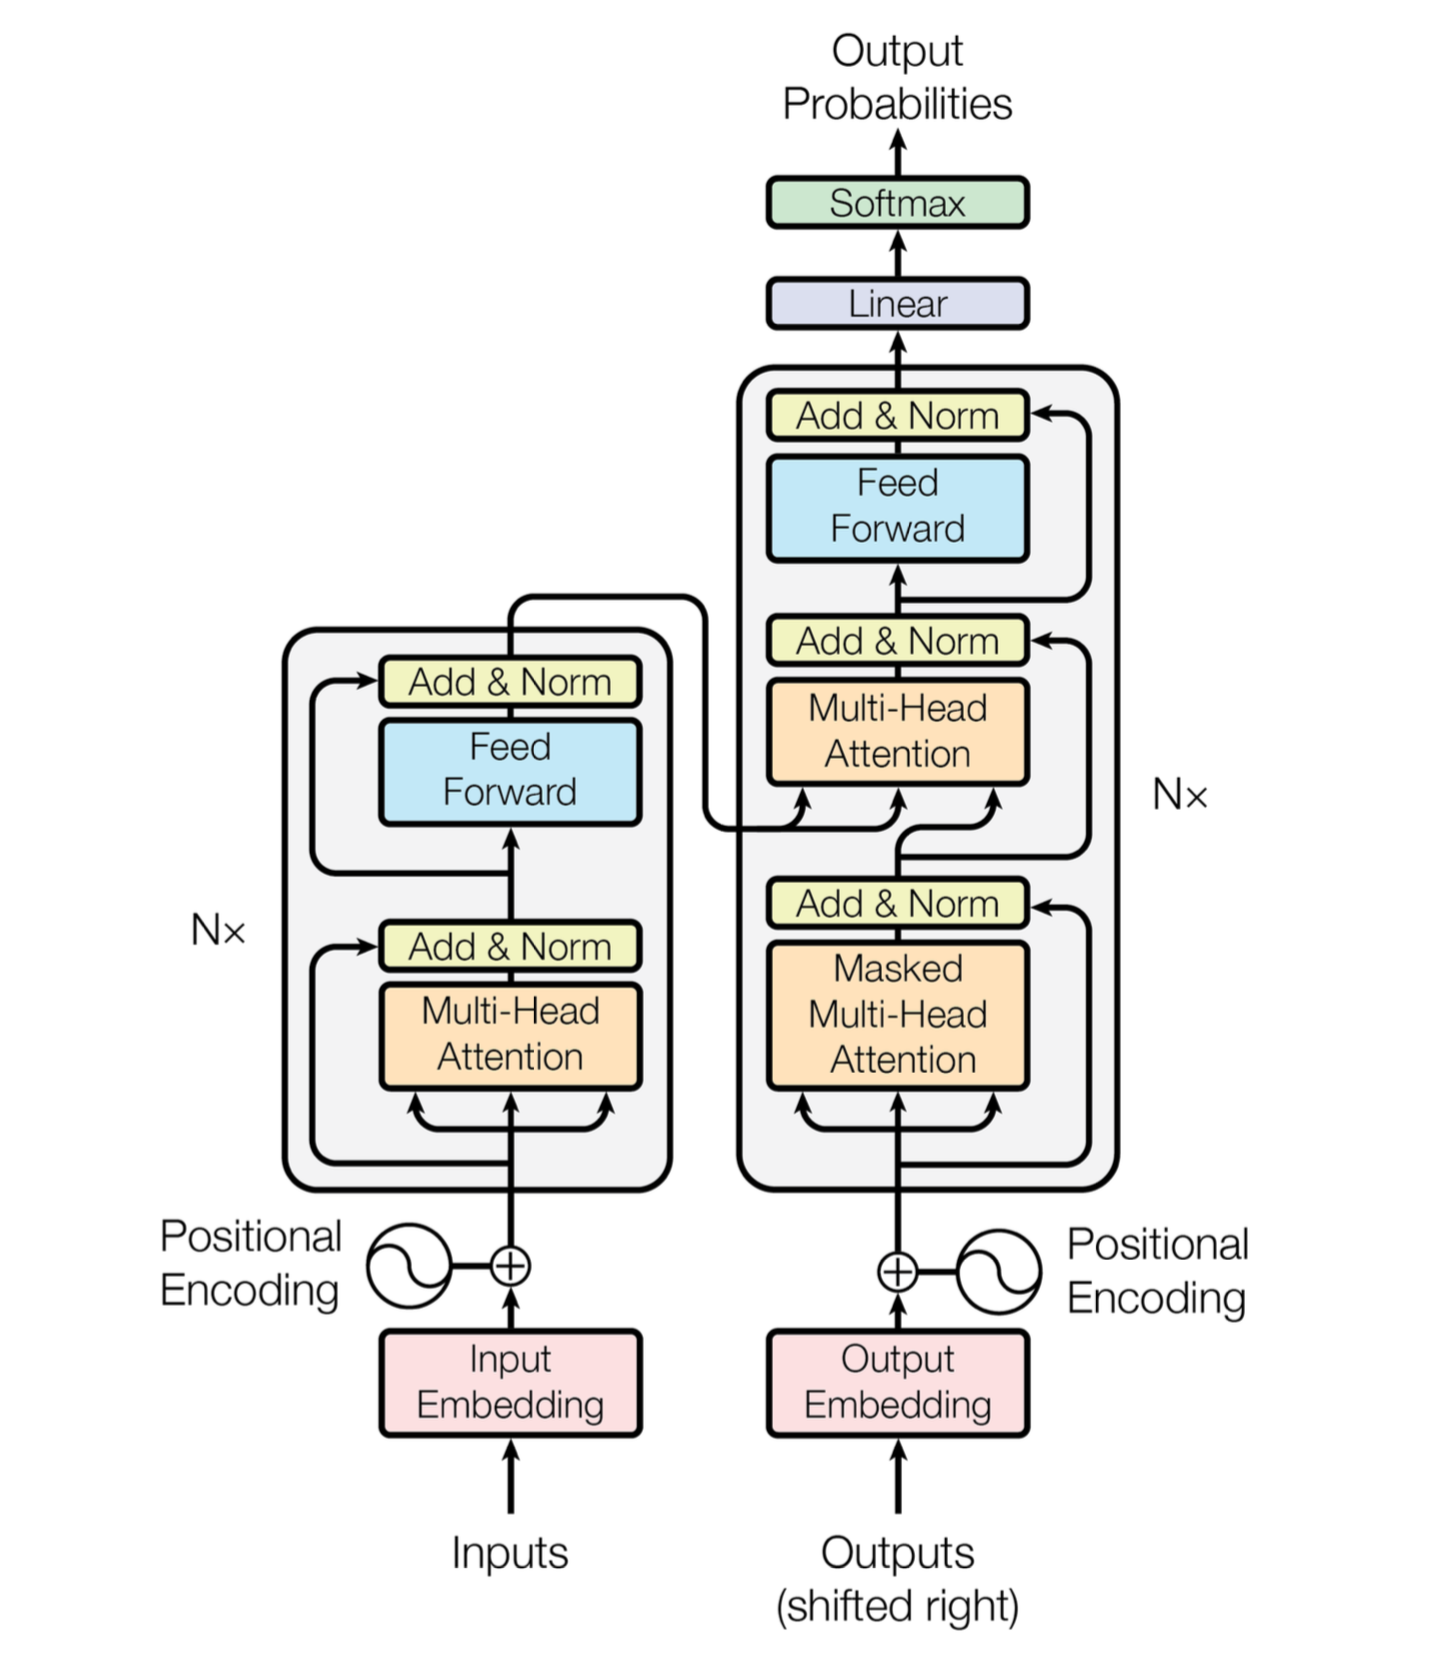
\includegraphics[height=12cm]{img/transformer}
  	\caption{Transformer model architecture}
	\label{fig:transformer}
\end{figure}
Figure~\ref{fig:transformer} shows the basic transformer architecture, which is fundamentally split up into the encoding stack on the left and the decoding stack on the right. A transformer block roughly consists of a self-attenntion (or multi-head-attention) layer, a layer normalization, a feedforward layer and finally another normalization layer. Residual connections are added before each normalization phase. Normalization and regularization techniques are commonly used to speed the training of deep models up and even improve their accuracy~\footcite{DBLP:journals/corr/abs-1903-00925}. After determining the input and output embeddings there is a preliminary step called \textbf{positional encoding}. As stated above, transformers do not contain recurrence or convolution. So, in order for the model to understand the ordering of the input sequence, information about either the relative or absolute position of the tokes in the sequence need to be injected. These positional encodings have the same dimension as the embeddings, so the two can be summed. The encodings are hereby not learned, but take on the form of some function $ f: \mathbb{N} \rightarrow \mathbb{R}^k $ to map the positions to real valued vectors. For the original transformer, sine and cosine functions of different frequencies were utilized:
\begin{align}
	\begin{split}
		PE_{pos, 2i} = \text{sin} \ \left( \text{pos} \ / 10000^{2i / k} \right) \\
		PE_{pos, 2i + 1} = \text{cos} \ \left( \text{pos} \ / 10000^{2i / k} \right)
	\end{split}
\end{align}
These functions were chosen, as the researches hypothesized that they would allow the model to easily learn to attend by relative positions, since for any fixed offset $ o $, $ PE_{pos + k} $ can be represented as a linear function of $ PE_{pos} $. Another advantage of choosing functions rather than learning positional embeddings stems from the fact that the model can learn to extrapolate to sequence lengths longer than the  ones encountered during training. After calculating the embeddings, adding the positional encodings and passing the encoder and decoder stacks, a learned linear transformation is used and afterwards a softmax function applied to convert the decoder output to predicted next-token probabilites. In order to actually predict the next word, a sampling strategy needs to elect one from the final probability distribution.

